% figs/actuation_modes_tikz.tex
\documentclass[tikz]{standalone}
% Common TikZ styles (standalone, robust)
\usetikzlibrary{arrows.meta,positioning,fit,calc,shapes,decorations.markings}

% 予約キー衝突や引数取りこぼしを避けるため分割宣言
\tikzset{every picture/.style={line cap=round, line join=round}}
\tikzset{box/.style={draw, rectangle, rounded corners,
  minimum width=2.2cm, minimum height=0.9cm, align=center, very thick}}
\tikzset{arrow/.style={-{Stealth}, very thick}}
\tikzset{line/.style={draw, very thick}}
\tikzset{dashedline/.style={draw, dashed, thick}}

% "node" は再定義しない。点用スタイルは独自名を使う
\tikzset{point/.style={circle, draw, minimum size=5.5mm, inner sep=0pt, thick}}

% 小さな実線ドット(Fig.2 が使う)
\tikzset{dot/.style={circle, fill, inner sep=0pt, minimum size=2.2pt}}

\tikzset{group/.style={draw, rounded corners, inner sep=5pt, thick}}
\tikzset{small/.style={font=\footnotesize}}
\tikzset{note/.style={rectangle, draw, fill=yellow!18, rounded corners,
  inner sep=2.5pt, font=\scriptsize\sffamily, thick}}
 % 共通スタイル
\begin{document}
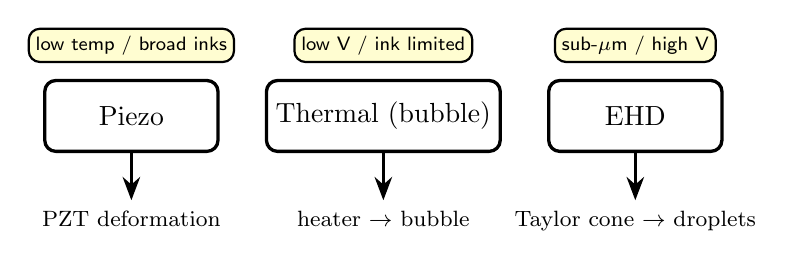
\begin{tikzpicture}[x=3.2cm,y=1cm]
  % Piezo
  \node[box] (piezo) at (0,0) {Piezo};
  \node[note,above=2mm of piezo.north] {low temp / broad inks};
  \draw[arrow] (piezo.south) -- ++(0,-0.6) node[below,small]{PZT deformation};

  % Thermal
  \node[box] (thermal) at (1,0) {Thermal (bubble)};
  \node[note,above=2mm of thermal.north] {low V / ink limited};
  \draw[arrow] (thermal.south) -- ++(0,-0.6) node[below,small]{heater $\to$ bubble};

  % EHD
  \node[box] (ehd) at (2,0) {EHD};
  \node[note,above=2mm of ehd.north] {sub-$\mu$m / high V};
  \draw[arrow] (ehd.south) -- ++(0,-0.6) node[below,small]{Taylor cone $\to$ droplets};
\end{tikzpicture}
\end{document}
